\section{Глава 1. Постановка задачи оценки параметров сигнала с расширенным спектром. Оценка источника сигнала на фоне АБГШ}

\subsection{Система с ШПС}
В данной работе рассматриваются задачи повышения рабочих характеристик приемников широкополосного сигнала, на примере СНС Navstar GPS,
поэтому целесообразно отразить основные модули этой системы - рисунок \ref{pic:sec1_gnss_system}.
\begin{figure}[H]
	\center\scalebox{1}{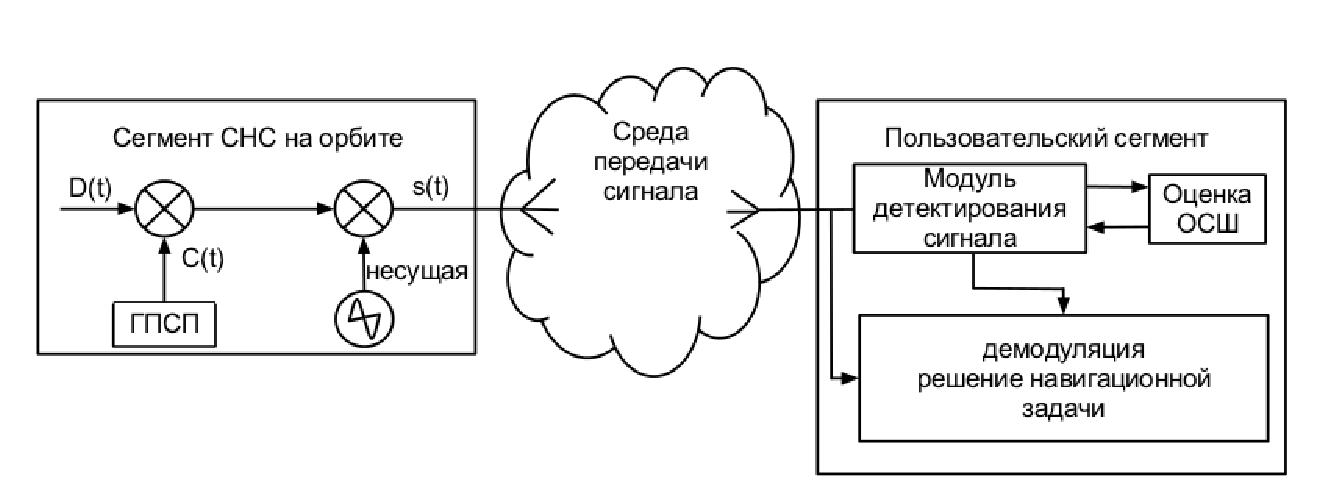
\includegraphics[width=1\linewidth]{sec1gnss_system.eps}}
	\caption{структутраная схема СНС GPS}
	\label{pic:sec1_gnss_system}
\end{figure}

В систему СНС Navstar GPS входят космический сегмент, наземный сегмент (на рисунке \ref{pic:sec1_gnss_system} не
отражен), а так же пользовательский сегмент. В космический сегмент входит спутниковая группировка, в 
наземный - станции управления, в пользовательский - все устройства принимающие сигнал от СНС Navstar GPS.

В системе СНС Navstar GPS применяется ШПС. Система передачи информации считается системой с расширенным спектром в следующих случаях \cite{sklyar}:
\begin{enumerate}
	\item Используемая полоса значительно шире минимальной, необходимой для передачи данных.
	\item Расширение спектра производится с помощью так называемого расширяющего сигнала (ПСП),
		который не зависит от передаваемой информации.
	\item Восстановление исходных данных ("сужение спектра") осуществляется путем сопоставления полученного
		сигнала и синхронизированной копии расширяющего сигнала (ПСП)
\end{enumerate}

Так же подобные сигналы называют:
\textquotedblleftсложными\textquotedblright,
\textquotedblleftшумоподобными\textquotedblright,
\textquotedblleftпсевдослучайными\textquotedblright,
\textquotedblleftсложными-дискретными\textquotedblright,
\textquotedblleftдискретно-кодированными\textquotedblright,
\textquotedblleftортогональными (квазиортогональными)\textquotedblright,
\textquotedblleftоптимальными дискретными\textquotedblright
\cite{gantmaher-book}.

Каждое название ставит акцент на определенной характеристике сигнала. В данной работе я буду оперировать термином
широкополосный сигнал - ШПС. ШПС можно определить как \cite{gantmaher-book, varakin-book}:
\begin{center}
\begin{equation}
	\label{eq:ss_signal}
	1 << FT = B,
\end{equation}
\end{center}
где: ${B}$ - база сигнала, ${F}$ - эффективная ширина спектра, а ${T}$ - длительность.
Неточность этого определения рассмотрена в \cite{gantmaher-book}, так же там даны ссылки на другие источники
разделяющие критику данного определения. Для данной работы критика, рассмотренная в приведенных источниках,
принципиального значения не имеет.

\subsection{Сигнал на выходе модулятора. Свойства применяемой ПСП}
В диссертации рассматривается сигнал с расширенным спектром полученный методом "прямой последовательности".
Данный метод заключается в том, что гармоническая несущая сигнала модулируется высокоскоростным (широкополосным)
расширяющим сигналом. 

Несущее колебание с частотой ${\omega_0}$  модулируется данными ${d(t)}$ , а также высокоскоростной ПСП ${g(t)}$, полученной методом "прямой последовательности".
СПИ Navstar GPS осуществляется двоичная фазовая модуляция (ДФМ или 2-ФМ), а значит ${d(t)}$  и ${g(t)}$  - потоки антиподных импульсов \{-1, 1\}. На рисунке 
\ref{pic:bit_and_code} представлены данные и модулирующая последовательность на длине 1 бита ${T_b}$.
\begin{figure}[H]
	\center\scalebox{0.5}{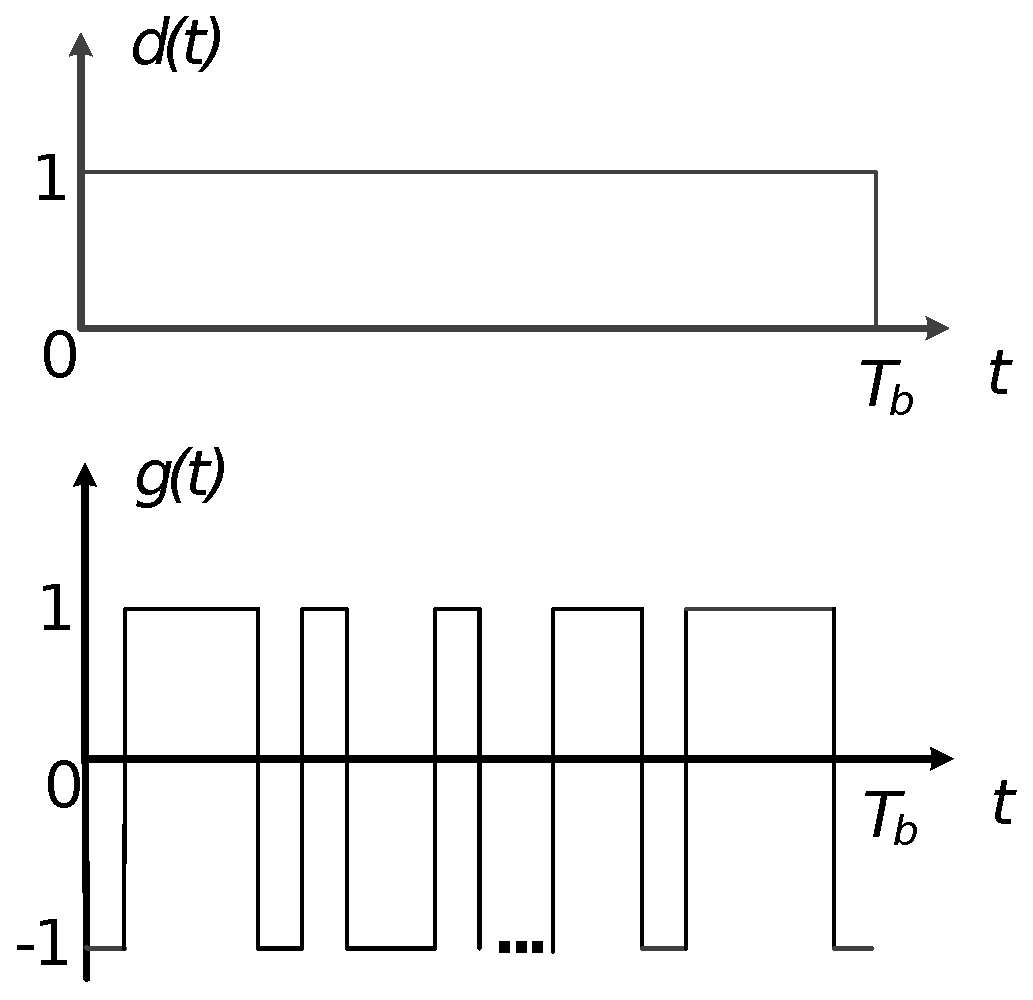
\includegraphics[width=1\linewidth]{bit_and_code.eps}}
	\caption{Информационный бит ${d(t)}$ и модулирующая последовательность ${g(t)}$ } 
	\label{pic:bit_and_code}
\end{figure}

Таким образом сигнал на выходе модулятора может быть представлен \cite{shahtarin_sync}:
\begin{equation}
	\label{eq:cdma_eq}
	s(t)=Ad(t)g(t)\cos{(\omega_{0}t)},
\end{equation}
где ${A}$ - амплитуда, ${d(t)}$- информационный бит, а ${g(t)}$ - ПСП.

Как уже было отмечено, в данной работе рассматривается ШПС полученный методом прямой последовательности. При данном методе
расширения спектра достигается за счет модуляции несущей частоты чаще всего двоичной ПСП или за счет псевдослучайной перестройки рабочей частоты \cite{borisovBook}.
Рассматриваемое в работе семейство ПСП Голда относится к ПСП, модулирующей сигнал при помощи псевдослучайной перестройки рабочей частоты - ФМШПС. Так как в данной работе
не рассматриваются другие виды ПСП, будем заменять термин ФМШПС термином ШПС, принимая во внимание только случай ФМШПС.
Таким образом \ref{eq:cdma_eq} может быть также записано как:
\begin{equation}
	\label{eq:cdma_eq_phi}
	s(t)=Ad(t)\cos{(\omega_{0}t + \theta_k)},
\end{equation}
где ${(\theta_k=\alpha_k \pi, \alpha_k \in \{0, 1\})}$

Информационный бит ${d(t)}$ остается постоянным в течении промежутка ${T_b}$:
\begin{equation}
	\label{eq:cdma_eq_data}
	 d(t) = \begin{cases}
		1, 0 \le t \le T_b \\
		0, t \not\in [0, T_b]
		\end{cases}
\end{equation}

В случае прямоугольной формы символов информационной последовательности двоичной ШПС на длительности одного бита данных можно представить как:
\begin{equation}
	\label{eq:cdma_eq_phi}
	s(t)=Ad(t)g(t)\cos{(\omega_{0}t + \theta_0)}, 0 \le t \le T_b,
\end{equation}
где ${\theta_0}$ - начальная фаза сигнала, ее значение имеет равномерное распределение на интервале ${(\theta_0 \in [0, 2\pi])}$.

Известно, что для случайной последовательности (СП) корреляционная функция (КФ) равна:
\begin{equation}
	\label{eq:cdma_ca_corr_func}
	 R_p(\tau) = \begin{cases}
		1 - \frac{|\tau|}{\tau_c}, |\tau| < \tau_c; \\
		0, |\tau| > \tau_c.
		\end{cases}
\end{equation}

График КФ СП приведен на рисунке \ref{pic:cf_code}.
\begin{figure}[H]
	\center\scalebox{0.7}{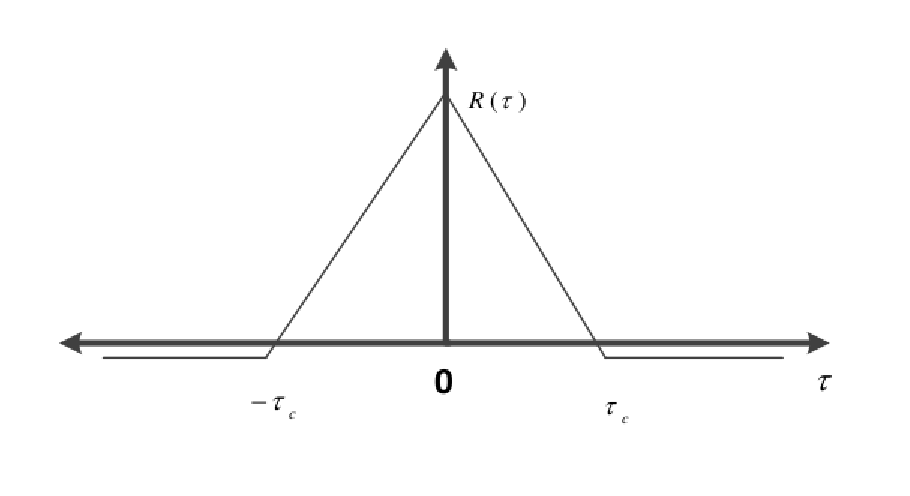
\includegraphics[width=1\linewidth]{cf_code.eps}}
	\caption{График КФ СП} 
	\label{pic:cf_code}
\end{figure}

СПМ ${G_p(f)}$ центрированного СП по теореме Винера-Хинчина является преобразованием Фурье
от КФ \cite{borisovBook}:
\begin{center}
\begin{eqnarray}
	\label{eq:psd_corr_func}
	G_p(f) & = & \int^{\inf}_{inf} R(\tau)e^{-j2\pi f \tau} d\tau = \int^{\inf}_{inf} \left( 1 - \frac{|\tau|}{\tau_c} \right) e^{-j2\pi f \tau} d\tau = \nonumber \\
		& = & \int^{\tau_c}_{0}\left( 1 - \frac{|\tau|}{\tau_c} \right) \cos{(2\pi f \tau)} d\tau = \tau_c \left( \frac{\sin{(\pi f \tau_c)}}{\pi f \tau_c} \right)^2
\end{eqnarray}
\end{center}

Выражение \ref{eq:psd_corr_func} представляет собой СПМ произведения ${p(t)d(t)}$ при использовании случайного сигнала ${p(t)}$.

\subsection{Оценка параметров}
Из литературы по теории автоматических систем, например \cite{pugachev} (глава 10.1), известна классическая постановка
задачи задачи теории оптимальных систем. "На практике часто приходится решать задачу проектирования системы, когда
требуется определить характеристики системы таким образом, чтобы она имела наибольшую точность при данных условиях.
Систему обеспечивающую наибольшую возможную точность с какой-нибудь определенной точки зрения среди всех систем
заданного класса, обычно называют оптимальной" \cite{pugachev}.

В одной из постановок данной задачи \cite{pugachev} (глава 10.1), система считается полностью неизвестной
и требуется определить ее оператор так, чтобы она была оптимальной с точки зрения принятого критерия качества. Эта
задача сводится к определению с наибольшей возможной точностью некоторых параметров, от которых зависит принимаемый
сигнал. Но при этом важно учитывать не только точность, но и другие факторы, так как проектируемая система должна
удовлетворять многим, часто противоречивым требованиям. В виду приведенных факторов, обычно представляет собой
ряд компромиссных решений, удовлетворяющих всем предъявляемым к системе требованиям.

Точность автоматической системы обычно характеризуется математическим ожиданием и дисперсией ее ошибки.
Математическое ожидание представляет собой систематическую ошибку системы в данных условиях, а дисперсия
характеризует уровень случайных ошибок \cite{pugachev} (глава 10.2). Так как в различных условиях работы
системы, которые встречаются случайно систематическая ошибка тоже является случайной, за критерий качества
системы при ее проектировании обычно принимают второй начальный момент ошибки - математическое ожидание
квадрата ошибки:
\begin{center}
\begin{equation}
	\label{eq:stat_err_prob}
	\eta = M[e^2(t)]
\end{equation}
\end{center}
Положительный квадратный корень из этой величины называют средней квадратичной ошибкой системы. Таким образом,
оптимальной системой обычно считают такую систему, которая имеет минимальную среднюю квадратичную ошибку.

Критерий минимума средней квадратичной ошибки является простейшим с математической точки зрения и обычно приводит
к наиболее простым методам определения оптимальных систем. Следует отметить, что далеко не во всех задачах он может служить мерой
качества системы. 

В случаях, когда необходимо проектировать следящую систему, приходится учитывать возможность срыва слежения,
который заключается в том что система перестает работать, если ее ошибка превосходит по абсолютной величине некоторый
уровень. При проектировании таких систем целесообразно принять за критерий качества вероятность срыва слежения. При
этом оптимальной считается такая система, которая обеспечивает минимум вероятности срыва слежения. Если срыв слежения
происходит в случае, когда абсолютная величина ошибки превосходит уровень $a$, то критерий минимума вероятности ошибки
слежения можно представить \cite{pugachev} (глава 10.2):
\begin{center}
\begin{equation}
	\label{eq:prob_lost_signal}
	p = P(e(t) > a) = min
\end{equation}
\end{center}

\subsection{Задача оценки параметров ШПС}

\subsection{Алгоритм оптимальной оценки параметров ШПС}
Алгоритм реализующий метод максимального правдоподобия - последовательный коррелятор. Данный подход реализуется в аппаратных приемниках.
Аппаратный приемник позволяет реализовать параллельно несколько последовательных корреляторов и вести оценку параметров
СПИ с ШПС параллельно.

Данный алгоритм в некоторых источниках так же называется согласованным фильтром. В \cite{sklyar} рассмотрены нюансы этих двух понятий.
В данной работе используется понятие последовательный коррелятор. Работа коррелятора описывается математической операцией
корреляции \ref{eq:serial_corr}. Сигнал коррелируется с локальной копией и на выходе коррелятора получается значение, отражающее
степень совпадения сигналов. Не трудно представить, что сигнал с хорошими корреляционными свойствами должен обладать высоким значением
корреляции когда сигналы синхронизированы и минимальным значением в любом другом случае (фаза ПСП не выровнена - отсутствие сигнала).
\begin{equation}
	\label{eq:serial_corr}
	y(m)=\sum\limits_{n=0}^{N-1}{x(n)h(m+n)},
\end{equation}
где ${x(n)}$ - принятая смесь, а ${h(m)}$ не импульсная характеристика системы, а локальная копия сигнала.

%%%%%%%%
% DFT

Вычисление циклической свертки через дискретное преобразование Фурье (ДПФ) - достаточно популярный метод
в программных приемниках, так как позволяет существенно уменьшить количество операций при вычислении. Как показано
в \cite{tsui, oppenheim}, можно достаточно просто перейти от свертки к циклической корреляции. Так как этот метод является самым
популярным в программных приемниках стоит его представить.
Свертка может быть представлена как:
\begin{equation}
	\label{eq:fft_conv}
	y(m)=\sum\limits_{n=0}^{N-1}{x(n)h(m-n)}
\end{equation}

Стоит отметить, что в \ref{eq:fft_conv} сдвиг во времени является циклическим, поскольку дискретные операции являются циклическими.
Возьмем ДПФ от \ref{eq:fft_conv}
\begin{center}
\begin{eqnarray}
	\label{eq:fft_conv_fft}
	Y(k) & = & \sum\limits_{n=0}^{N-1}\sum\limits_{m=0}^{N-1}{x(m)h(n-m)e^{(-j2\pi{kn})/N}}=\nonumber \\
	& = & \sum\limits_{m=0}^{N-1}{x(m)}[\sum\limits_{n=0}^{N-1}h(n-m)e^{(-j2\pi{(n-m)}k)/N}]e^{(-j2\pi{m}k)/N}=\\
	& = & H(k)\sum\limits_{m=0}^{N-1}e^{(-j2\pi{m}k)/N} = X(k)H(k)\nonumber 
\end{eqnarray}
\end{center}
Из уравнения \ref{eq:fft_conv_fft} легко видеть, что это не линейная свертка. В линейной свертке для входного сигнала размером в ${N}$ точек,
результат будет из ${2N-1}$ точек. А в уравнении выше, результатом является всего ${N}$ точек.
Это проявление циклической природы ДПФ.

Алгоритм оценки не использует свертку, он использует корреляцию, которая отличается от свертки. Корреляция
между $x(m)$ и $h(m)$ записывается выражением \ref{eq:serial_corr}:
Единственным отличаем между \ref{eq:serial_corr} и \ref{eq:fft_conv} является знак перед $n$ в ${h(m+n)}$.
В случае оценки параметра ШПС, $h(m)$ является локальной копией сигнала, а не импульсной характеристикой.
\begin{center}
\begin{eqnarray}
	\label{eq:fft_corr_fft}
	Z(k) & = & \sum\limits_{n=0}^{N-1}\sum\limits_{m=0}^{N-1}{x(m)h(n+m)e^{(-j2\pi{kn})/N}}=\nonumber \\
	& = & \sum\limits_{m=0}^{N-1}{x(m)}[\sum\limits_{n=0}^{N-1}h(n+m)e^{(-j2\pi{(n+m)}k)/N}]e^{(j2\pi{m}k)/N}=\\
	& = & H(k)\sum\limits_{m=0}^{N-1}e^{(j2\pi{m}k)/N} = X(k)H^{-1}(k)\nonumber 
\end{eqnarray}
\end{center}
где ${X^{-1}(k)}$ - обратное ДПФ. Уравнение \ref{eq:fft_corr_fft} можно записать как:

\begin{equation}
	\label{eq:fft_corr_fft_rev}
	Y(k) = \sum\limits_{n=0}^{N-1}\sum\limits_{m=0}^{N-1}{x(n+m)h(m)e^{(-j2\pi{kn})/N}}=X^{-1}(k)H(k)
\end{equation}

Если сигнал $x(n)$ действительный, то $x(n) = x^*(n)$, где ${^*}$ - операция комплексного сопряжения. Используя данное соотношение,
значение $Z(k)$ может быть записано:
\begin{equation}
	\label{eq:fft_magnitude}
	|Z(k)|=|H^*(k)X(k)|=|H(k)X(k)^*|
\end{equation}
Данное соотношение может быть использовано для нахождения значения циклической корреляции между входным сигналом и 
локальной копией.

\subsection{Алгоритм оценки параметров ШПС на фоне АБГШ c использованием АР модели}

%%%%%%%%%%%%%%%%%%%%%%%%%%%%%%%%%%
%В реальных СПИ сигнал на приемник поступает одновременно от нескольких источников, присутствует неопределенность по частоте, а также аддитивный белый шум (АБГШ).
%В приемнике после оцифровки сигнала получаем смесь:
%\begin{equation}
%	\label{eq:cdma_strip_eq}
%	x(m)=\sum_{k=1}^{N}\left( A_k g(m + \tau_k)\exp{\left[j \left( \tilde{\omega}_{k}m + \phi_k(m)\right)\right]} \right) + n(m),
%\end{equation}
%где  ${k}$ - относительный номер источника сигнала, ${N}$ - количество доступных источников сигнала, модулированных ПСП одного семейства,
%${m}$ - индекс соответствующий времени, ${\tilde{\omega}_{k}}$  – относительная частота, соответствующая ${\omega_0}$,
%${\tau_k}$ - задержка модулирующей ПСП в точке приема, ${\phi_k(m)}$ - случайная начальная фаза, ${n(m)}$ - аддитивный белый гауссов шум (АБГШ). 
%
%Следует отметить, что при оценке фазы сигнала с номером ${k}$  интерференцией являются сигналы:    .
%\begin{equation}
%	%\label{eq:cdma_interference}
%	\{n \ne k, n \in [1,N]\}
%\end{equation}

%\subsection{Постановка задачи оценки параметров сигнала с расширенным спектром}
%\paragraph{Основные свойства широкополосных сигналов}
%
%%%%%%%
%\paragraph{Классическая постановка задачи оценки параметра.}
%
%%%%%%%
%%%%%%%
%\paragraph{Алгоритмы оценки параметров широкополосного сигнала сигнала.}
%
%%%%%%%%%
%% Chaos 
%Оценка параметров СПИ с ШПС (в частности сигналов системы Navstar GPS) с помощью осциллятора Дуффинга
%достаточно новое направление в исследованиях по данной тематике. В данной области опубликовано несколько работ, в частности \cite{chaos_chen, chaos_cambridge, chaos_huang, chaos_song}.
%Так же является интересной более ранняя статья не рассматривающая GPS \cite{chaos_wang}.
%Осциллятор Дуффинга с гармоническим внешним воздействием может быть описан уравнением:
%\begin{center}
%\begin{equation}
%	\label{eq:duffing}
%	mx'' + cx' + k_{1}x + k_{2}x^3 = F_{0}\cos(\omega{t}),
%\end{equation}
%\end{center}
%где $m$ - масса, $c$ - коэффициент диссипации, $x$ - состояние осциллятора, $k_1$ и $k_2$ - линейный и нелинейный коэффициенты соответственно,
%$F_{0}\cos(\omega{t})$ - внешнее воздействие.
%
%Подробно уравнение \ref{eq:duffing} рассмотрено в \cite{chaos_neimark_landa}.
%Для использования осциллятора Дуффинга с целью оценки параметров ШПС была предложена усовершенствованная форма \cite{chaos_song, chaos_chen}:
%\begin{center}
%\begin{equation}
%	\label{eq:duffing_gps}
%	x'' +cx' - x^3 + x^5 = \gamma\cos(\omega{t}) + (\gamma_{x}\cos(\omega_{x}) + n(t))
%\end{equation}
%\end{center}
%
%Перепишем динамическую систему \ref{eq:duffing_gps} в виде:
%\begin{center}
%\begin{equation}
%	\label{eq:duffing_gps_2}
%	\left\{
%	\begin{aligned}
%		y(t) & = x'(t) \\
%		y'(t) & =  -cx' + x^3 - x^5 + \gamma\cos(\omega{t}) + (\gamma_{x}\cos(\omega_{x}) + n(t)),
%	\end{aligned}
%	\right.
%\end{equation}
%\end{center}
%где ${n(t)}$ - АБГШ.
%
%Пример фазового портрета при ${\omega=\omega_{x}}$ изображен на рисунке \ref{pic:duffing_sync},
%фазовый портрет хаоса расположен на рисунках \ref{pic:duffing_chaos1}, \ref{pic:duffing_chaos2}
%\begin{figure}[H]
%	\center\scalebox{0.5}{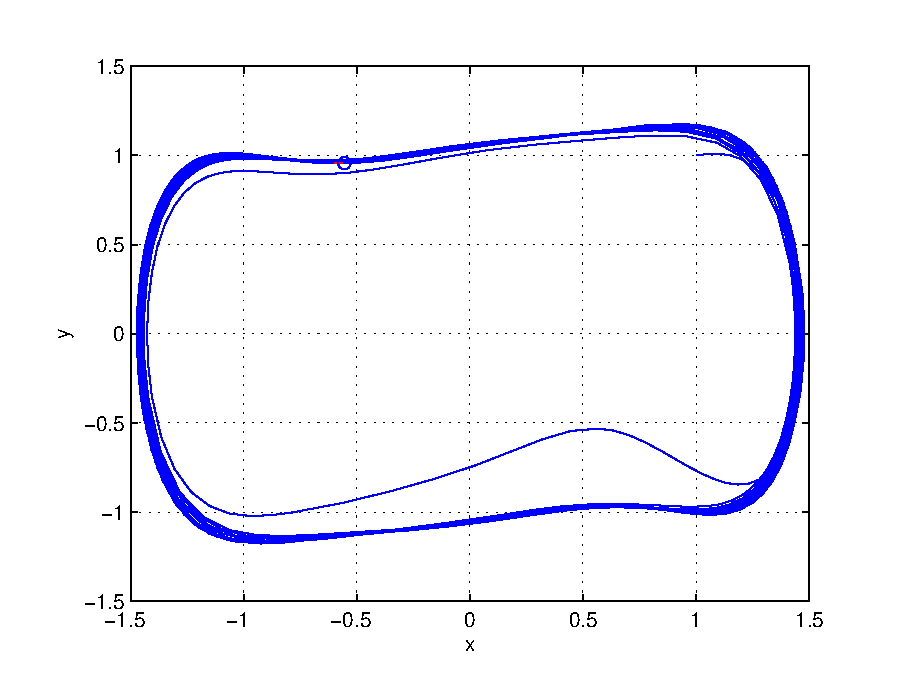
\includegraphics[width=1\linewidth]{duffing_sync.eps}}
%	\caption{Фазовый портрет при ${\omega =\omega_{x}}$}
%	\label{pic:duffing_sync}
%\end{figure}
%\begin{figure}[H]
%	\center\scalebox{0.5}{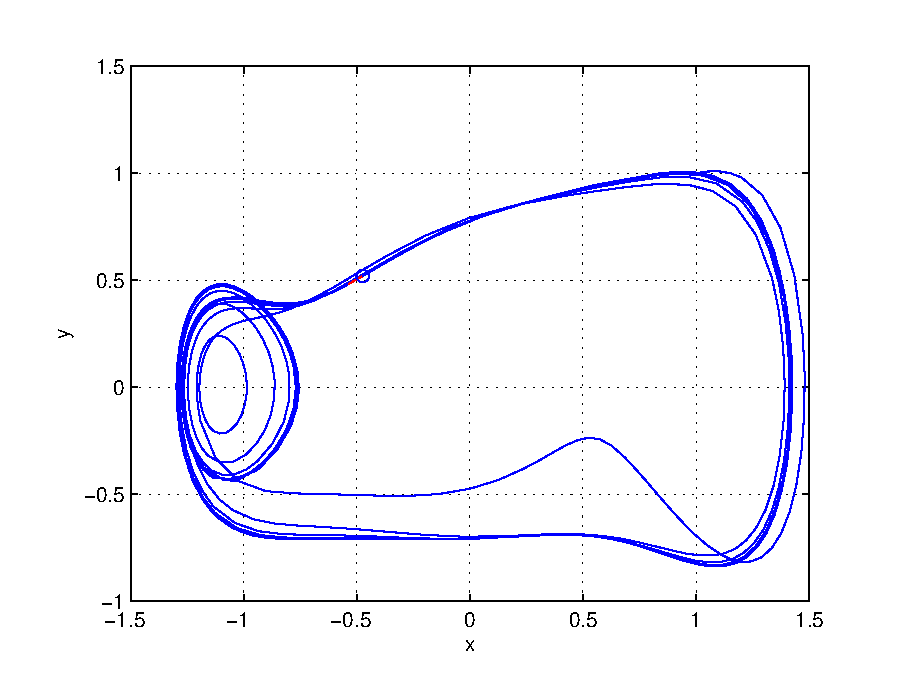
\includegraphics[width=1\linewidth]{duffing_chaos1.eps}}
%	\caption{Фазовый портрет при ${\omega < \omega_{x}}$}
%	\label{pic:duffing_chaos1}
%\end{figure}
%\begin{figure}[H]
%	\center\scalebox{0.5}{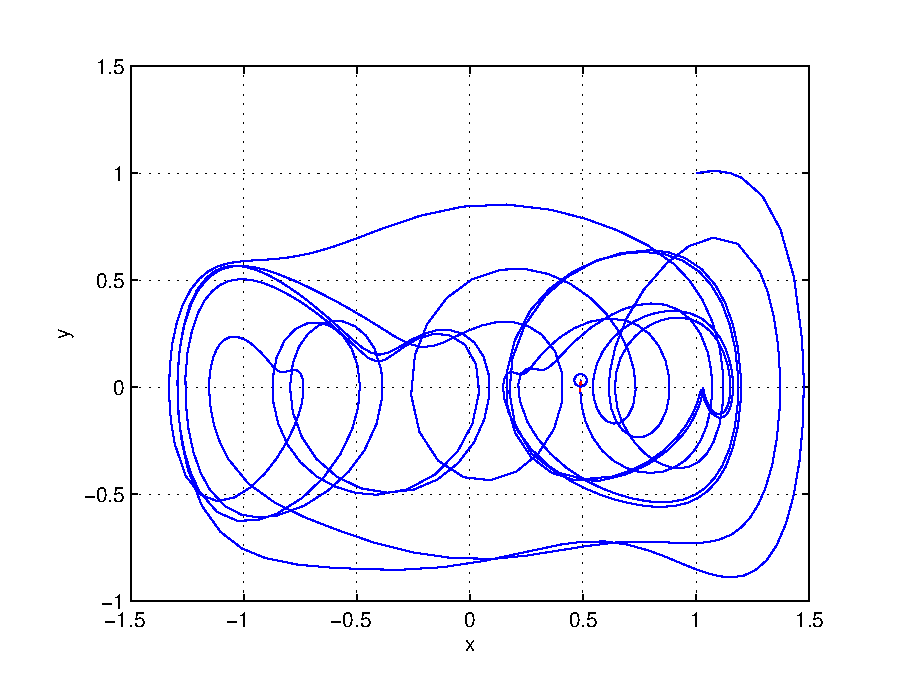
\includegraphics[width=1\linewidth]{duffing_chaos2.eps}}
%	\caption{Фазовый портрет при ${\omega > \omega_{x}}$}
%	\label{pic:duffing_chaos2}
%\end{figure}
%В качестве параметров уравнения применялись: $c = 0.5$, $\gamma=\gamma_{x}=0.36$, ${\omega=1}$
%
%Часто для вычисления характеристик хаотической динамики применяется показатель Ляпунова.
%Он показывает в каком состоянии находится система. Если система находится
%в стабильном состоянии линии фазовой траектории будут близко прилегать одна к другой, в противном
%случае система находится в состоянии хаоса. Детектор с применением показателя Ляпунова
%представлен на рисунке \ref{pic:chaos_lyapunov}.
%\begin{figure}[H]
%	\center\scalebox{0.7}{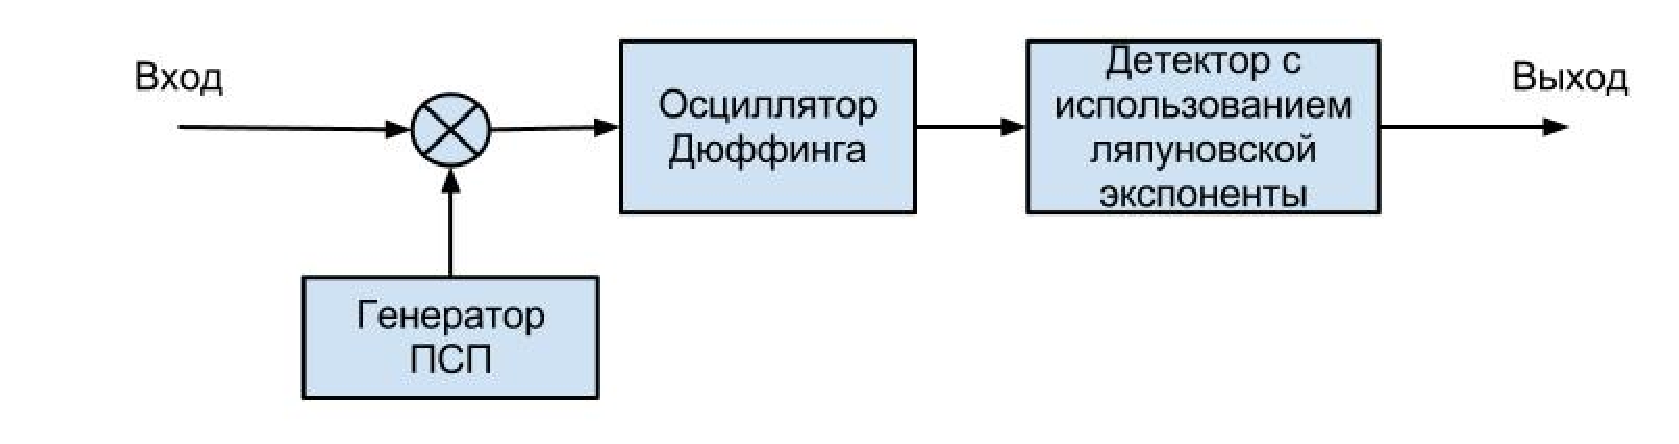
\includegraphics[width=1\linewidth]{Chaos_detector_Lyapunov.eps}}
%	\caption{Схема детектора основанного на показателе ляпунова для осциллятора Дуффинга}
%	\label{pic:chaos_lyapunov}
%\end{figure}
%
%В статье \cite{chaos_chen} предложен усовершенствованный метод, базирующийся на вычислении дисперсии
%фазовой траектории. Действительно, на рисунках \ref{pic:duffing_sync}, \ref{pic:duffing_chaos1},
%\ref{pic:duffing_chaos2} видно, что когда система находится в хаотическом состоянии значение
%дисперсии по координате ${x}$ больше, чем соответствующее значение в состоянии $\omega = \omega_{x}$.
%На основе этого была предложена усовершенствованная схема детектора сигнала - рисунок \ref{pic:chaos_energy_detector}
%\begin{figure}[H]
%	\center\scalebox{0.7}{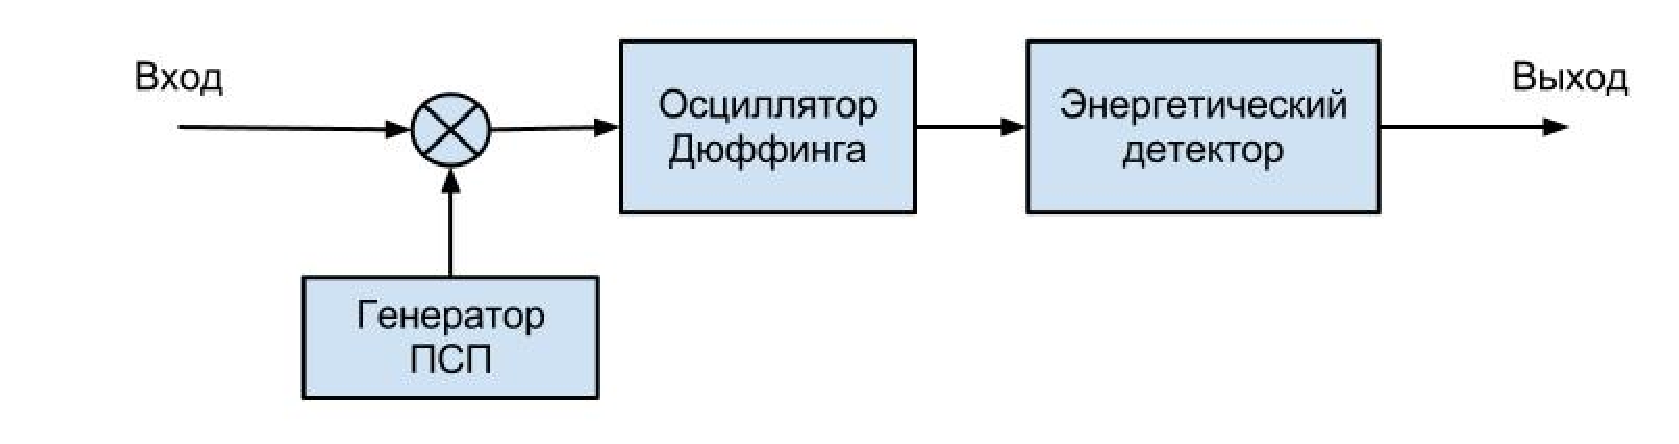
\includegraphics[width=1\linewidth]{chaos_detector.eps}}
%	\caption{Схема энергетического детектора для осциллятора Дуффинга}
%	\label{pic:chaos_energy_detector}
%\end{figure}
%
%%%%%%%%%
%% HOS 
%Математический аппарат статистик высоких порядков (СВП или HOS - Higher-order statistics)
%для исследования непричинных, причинных и нестабильных (систем с неминимальной фазой) и негауссовых сигналов впервые был предложен
%в \cite{hos_petropulu} в 1993 году.  Этот метод позволяет не только подавлять цветной Гауссов шум, но так же в некоторых случаях подавлять
%цветной не-Гауссов шум.
%
%В работе \cite{hos_zhao} был предложен метод детектирования ШПС с использованием СВП.
%
%%%%%%%%%
%% CHE 
%Интересная группа алгоритмов основывается на информационной избыточности ШПС, например \cite{phd_che}. В данной
%группе алгоритмов используется механизм появления нескольких точек на основном пике КФ, описанный в \cite{kaplan}. Пример
%изображен на рисунке \ref{pic:sec1_peak_tcd}.
%\begin{figure}[H]
%        \center\scalebox{1}{\includegraphics[width=1\linewidth]{corr_peak_tcd.eps}}
%        \caption{Идеальная КФ ШПС с отмеченными точками возможного обнаружения}
%        \label{pic:sec1_peak_tcd}
%\end{figure}
%На рисунке \ref{pic:sec1_peak_tcd} изображен пик КФ с несколькими точками. Две точки находятся выше порога ${\Pi=0.5}$.
%В работе \cite{phd_che} рассмотрено создание субоптимального обнаружителя на основе информационной избыточности ШПС.
%Получена целевая функция системы и намечены дальнейшие пути развития данного направления.
%
%%%%%%%%%
%% 2MAX 
%Так же одним из направлений исследований является разработка алгоритмов выбора порога без априорной информации о величине ОСШ. Например,
%в работах \cite{2max_ieee, 2max_article} представлен алгоритм нахождения пика (АНП) КФ (Peak-finding algorithm).
%
%Данный алгоритм можно разбить на несколько шагов:
%\begin{itemize}
%\item[Шаг 1] Подсчитать КФ, используя метод предложенный с использованием параллельного коррелятора. 
%\item[Шаг 2] Найти главный пик КФ, найти второй пик КФ, найти среднее значение КФ.
%\item[Шаг 3] Нормализовать полученные значения относительно главного пика КФ.
%\item[Шаг 4] Если (максимум КФ - среднее) > ${\Pi_1}$ и (максимум КФ - 
%	второй максимум КФ) > ${\Pi_2}$, тогда полученный главный пик КФ соответствует
%	искомой фазе ПСП и частоте.
%\end{itemize}
%
%В статье авторов \cite{2max_ieee} предложены следующие значения для порогов:
%${\Pi_1} = 0.3$ дБ и  ${\Pi_2} = 0.15$ дБ. Так же авторы предлагают итерационную процедуру для нахождения
%фазы ПСП и частоты смещения допплера:
%\begin{itemize}
%\item[Шаг 1] Начать вычисление с 1мс.
%\item[Шаг 2] Получить результаты АНП.
%\item[Шаг 3] Если фаза ПСП и частота не могут быть найдены, увеличить время интегрирования сигнала.
%	Использовать следующие значения для интегрирования: 1мс -> 10мс -> 50мс -> 100мс -> 200мс ->
%	500мс -> 1000мс
%\end{itemize}
%
%Очевидным минусом данного подхода является сильная зависимость от интерференции. В городском каньоне будет присутствовать
%несколько достаточно мощных лучей, а значит разница в энергии первого и второго пика будет низкой.
%
%%%%%%%
%\paragraph{Выводы.}
%
%Во введении кратко приведена история развития СПИ с ШПС, приведены ученые внесшие значительный вклад в разработку данного направления связи. Так же рассмотрена
%актуальность исследования в данной области. Кроме того, приведены определения, что такое СПИ с ШПС, ее математическая модель и основные отличительный особенности данного класса систем.
%Так же приведены классические и новые подходы к оценке параметров СПИ с ШПС. Рассмотрен оптимальный алгоритм - последовательный коррелятор,
%а так же новые достаточно экзотические подходы - применение осциллятора Дуффинга. 

\newpage
